\chapter{Relatório}

In this thesis an observer for an active prosthetic leg will be delevoped using an observer approach designed by Khalil. 
The observer has an adaptive gain related to joints signal-to-noise ratios.
The simulation step used in this thesis is 10Khz and a real-time controller with 1kHz sampling rate was considered in order to 
implement the real control signal.

In order to define a real SNR, one must consider the resolution error or the data provided on the datasheet.

\textbf{2018-07-09}


There 3 possible approaches for a SNR estimation:
1) Filter the raw signal in order to obtain a signal + noise

2) Create one more state, which will be regarded as disturbances

3) Empirical method

Tests with the SNR estimation algorithm showed that the Empirical method needs some improvements to be done, probably 
because it was designed for a different application.


\textbf{To be done}
\begin{itemize}
    \item Find the encoder used in the prosthetic leg and recreate the error signal distribution
    \item Improve the empirical method
    \begin{itemize}
        \item Avoid the spikes occurring during estimation
    \end{itemize}
    \item References
    \begin{itemize}
        \item \url{https://engagedscholarship.csuohio.edu/cgi/viewcontent.cgi?article=1014&context=etdarchive}
        \item journal of neuroengineering and rehabilitation
    \end{itemize}
\end{itemize}

\textbf{2018-07-11}

The main goal to use encoders instead of load cells for ground reaction forces estimation is to reduce weight and cost. 
As a drawback, a mathematical model of external forces needs to be designed. In Fakoorian, only joint angles are considered and that's a simplification 
for the case of a normal gait. If anything different from a flat ground appears, i.e. ramp or stair, the prosthetic 
user won't be able the take a step further.  The mathematical model for GRF estimation is a point of improvement and could also have motor currents as inputs.

Fakoorian was the first to propose an encoder as replacement for load cells as a GRF data device.

\textbf{To be done}
\begin{itemize}
    \item Describe types of prosthesis and main suppliers/developers
    \item Define an encoder resolution to use in the simulation with noise
    \item 
\end{itemize}

\textbf{2018-07-19}

Tests with lowpass filter have been done in order to estimate the output signal SNR. Firts of all, the input SNR has to be known so one could compare with 
a given SNR estiamtion. A simulation that considers quantization, noise and sampled-data implementation has been developed.

In order to define design a first order low-pass filter, the signal FFT has been calculated as depicted in \ref{fig:FFT_step}. Based on it, it has been 
concluded that a cutoff frequency in 30Hz would be enough to filter and provide an acceptable signal phase-shift. 
\begin{figure}[h]
    \centering
    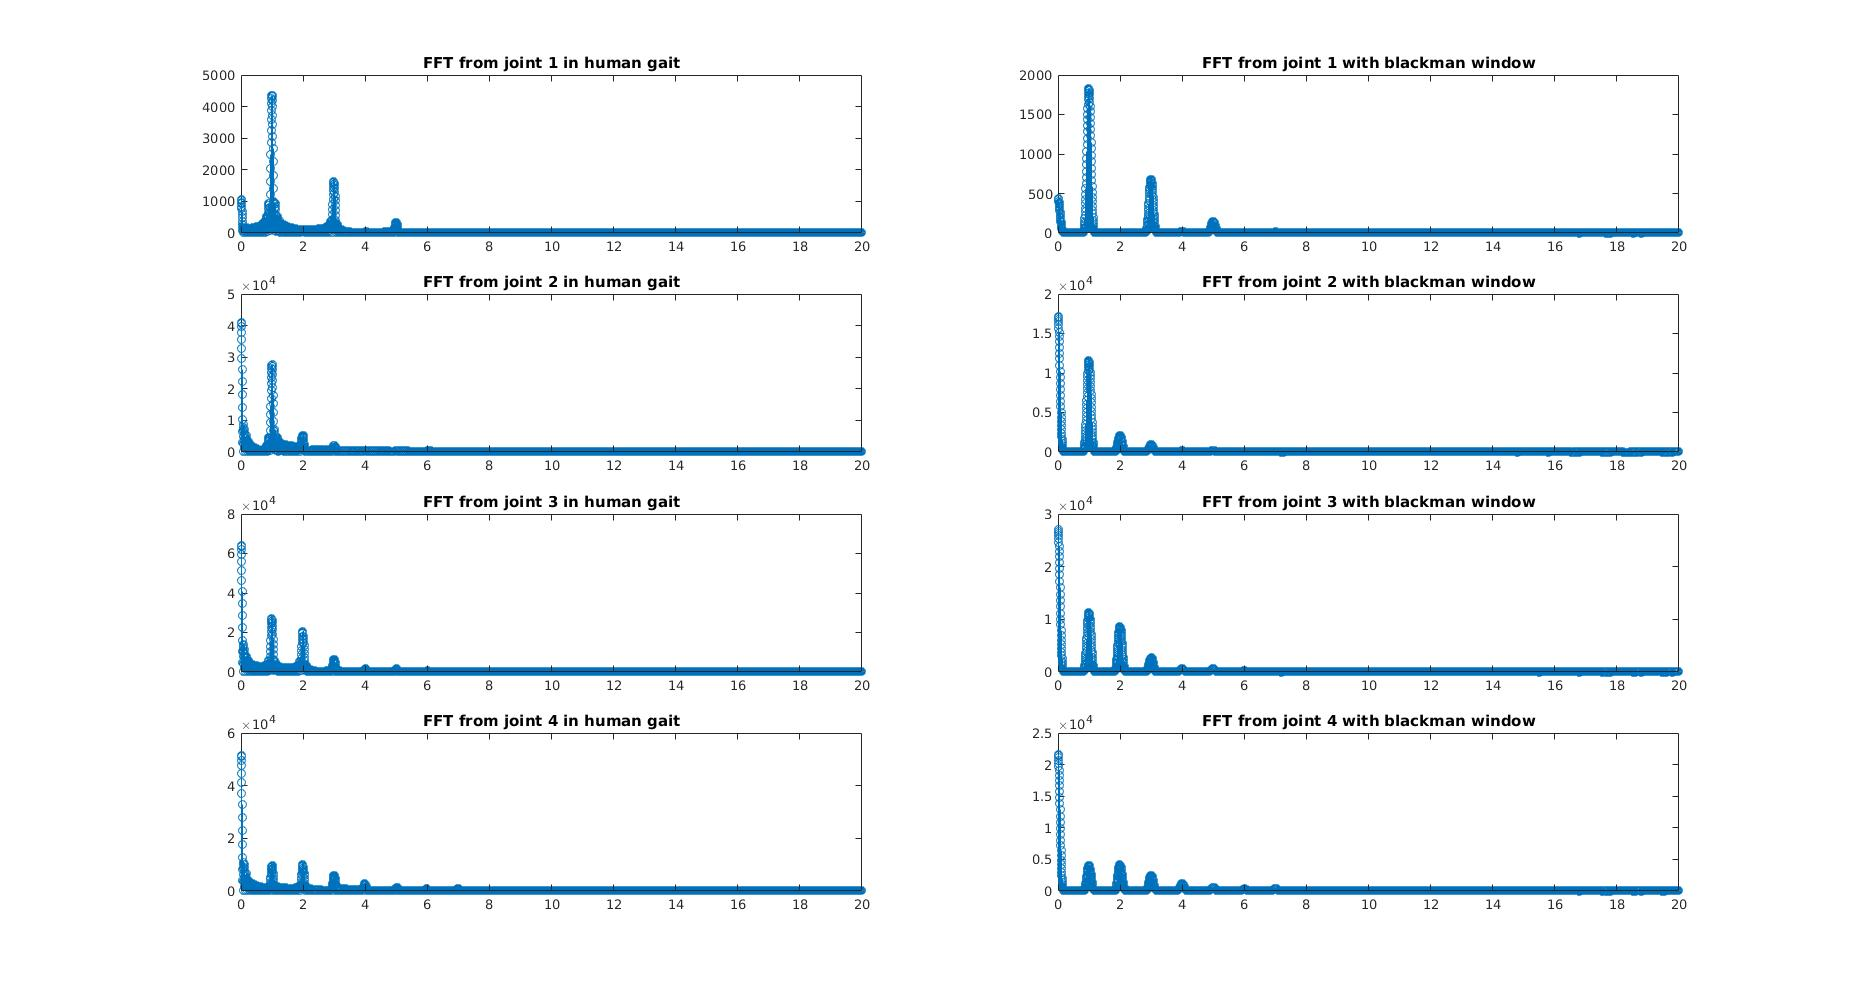
\includegraphics[width=\linewidth]{1sec_step_FFT.jpg}
    \caption{FFT example for Human gait considering a 1sec step}
    \label{fig:FFT_step}
\end{figure}

\textbf{2018-08-16}

Test with the first order filter will be carried on to validate it's implementation. First of all
it will be designed the filter with a cutoff frequency at 30Hz then an SNR algorithm will acquire the noise signal
by subtracting the raw\_signal from the filtered\_signal.

\textbf{2018-08-17}

A chapter for SNR estimation has been created. In that file the whole procedure for estimating SNR will be explained 

\textbf{2018-08-18}
The filter has been implemented and a the data was stored as \textit{data\_steps\_filtered}
The joint unit is an angle in radians. 

The results with the first order lowpass filter for a 15sec simulation were: due to a phase-shift of $[1.5079  1.4778  1.4745  1.5059]$ degrees, the filtered signal had a maximum joint error of $[1.14   6.35    12.03    9.17]$ degrees and the same SNR was obtained. 

Another implementation would be the empirical one using the script \textit{sinalruido.m}. 2 Bounderies are computed during the simulation, an upper and a lower one, in order to estimate a noise. The outputs from this script are $[SNR ruido upper lower noise]$ 

\textbf{2018-08-20}

The empirical approach was tested with some script changes. For the second joint an error of 7.3830 was obtained according to euclidian distance (norm command in Matlab) and a maximum 8.35 degrees error during a 5 seconds simulation.

\textbf{2018-08-24}

Considering an encoder resolution of 12 bits, the measurement precision is equal to $\frac{180}{\pi}.\frac{1}{2^{12}} = 0.014$, that means my quantization error would be more or less half my precision ($0.007$). Using the \textit{SNR\_mod.m}, it is possible to set the noise variance to 0.007 and acquire the noisy signal equivalent to that.

Today I had a meeting with Jacoud and we set some tasks about the thesis as follows:

\begin{enumerate}
    \item Run simulation with 4 joints tracking a reference signal (\textit{data\_steps}) with the states (from plant) and computed torque control without ground reaction forces
    \begin{enumerate}
        \item Create parametrical errors in matrix used for computed torque
    \end{enumerate}
    \item Run simulation with 4 joints tracking a reference signal (\textit{data\_steps}) with estimated states (from HGO) and computed torque control without ground reaction forces
    \item Implement 2 or 3 forms to estimate in open loop the SNR from signal control
    \begin{enumerate}
        \item Jacoud
        \item Low-pass (design filter using previous control signals)
    \end{enumerate}
    \item Implement a block in simulation that has error norm and SNR as inputs and a variable gain as output without ground reaction forces
\end{enumerate}

It is important to say the changes regarding the project. First of all, the SNR estimation will be used at the control signal instead of joint angles. It means that my control signal will have some high frequency components that will be filtered in order to smooth it. However, there is no a priori knowledge of its behavior. Therefore some samples will be needed in order to specify its frequency components.

Another change is regarding the rate trasition. As the simulation should increase its complexity according to some steps, the implementation of different sample frequencies for a real simulation will be postponed.

The first step today will be define every unit used in the system, as torque, angles, etc.

\begin{table}[h]
    \centering
    \begin{tabular}{|c|c|}
    \hline
    \multicolumn{2}{|c|}{Units Table} \\ \hline
    Torque            & Nm/s     \\ \hline
    Mass              & Kg       \\ \hline
    Subject length    & m        \\ \hline
    Joint angles      & rad      \\ \hline
    Force             & $m/s^{2}$\\ \hline
    \end{tabular}
\end{table}

After using the HGO states, remember to use a saturation block at the control signal, otherwise it will ``explode''.

\textbf{2018-08-26}

After simulating the first task (State Feedback), one could see that:
\begin{itemize}
    \item Initial state mismatch could lead to a transient response in the control signal
    \item 
\end{itemize}

\textbf{2018-08-27}

A simulation routine using the \textit{save} command  must be implemented in order to automate the parameters value change.

\textbf{2018-08-31}

After some trials, the need for correct control parameters was obvius. To do that the following control project was designed.

\begin{align}
M\ddot{\theta} + C\dot{\theta} + G &= \tau \\
\tau &:= C\dot{\theta} + G + \bar{\tau} \\
\bar{\tau} &:= M(u)\\
\ddot{\theta} &= u \\
e &= \theta - \theta_d \\
\ddot{e} &= u - \ddot{\theta_d} \\
u &:= \ddot{\theta_d} - K_pe - K_d\dot{e} - K_i\int_{t_o}^{t}e \, dt \\
\dddot{e} + K_d\ddot{e} + K_p\dot{e} + K_ie &= 0 \\
s^3 + K_ds^2 + K_ps + K_i &= 0 \\
(s^2 + 2\zeta \omega_n + \omega_n^2)(s + p) &= 0 \\
Ki &= \omega_n^2p \\
K_p &= \omega_n^2 + 2\zeta \omega_np \\
K_d &= p + 2\zeta \omega_n 
\end{align}

As the system's highest frequency component is 30Hz, $\omega_n > 2\pi30$. The damping factor will be arbitrarily chosen as $\zeta = 0.9$ and the pole should be faster than the $\omega_n$, therefore ... $3\omega_n$.


\textbf{2018-08-31}

The control input signal is saturating right in the beginning of the simulation. After some tests regarding dqInit and qInit conditions, it seems that the dirty derivative may be causing a high joinv velocity reference signal and this may cause $K_d\dot{e}$ to be a high value. This conclusion was taken after changing tau from 0.01 to 0.001 which gave the controller a better performance (reduced the tracking error from 0.1rad to 0.01 in PID)

One possible solution may be differentiating the data\_steps manually instead of applying durty derivative.

Now one must create the \textit{.mat} files with simulation results and then move to another step from the thesis (add parametrical error and then estimated states feedback)

Test with parametrical error have been implemented in \textit{Mass\_ctrl Inertia\_ctrl R\_ctrl L\_ctrl h\_ctrl} and both PD and PID control could handle it. After adding and error of $1 + 0.5*(rand()-1/2)$ the tracking error has the same peak values although the dynamic of it has changed.

During the implementation of HGO states feedback one could see that the control signal was saturating. That happened because the HGO gain $\mu$ was 0.0001, after changing its value to 0.001 the control signal had a better behaviour and the performance was the same.

\textbf{2018-09-01}

After noticing that the dirty derivative has its limitations, another approach to differentiate joint signals could be by curve fitting. That can be done using a matlab command called \textit{cftool}, in which one must enter the period and the signal, then choose the fitting curve that best suits the application. In this thesis case, the \textit{sum os sines} fit would be the best. For some joints the curve dynamics require more than 8 sines to be accurately represented, therefore this method was disregarded for now.

\textbf{2018-09-04}

Today the focus was on Empirical SNR Estimation method. After some problems regarding the superior and inferior buffer, one could conclude that as the buffers are declared as global variables then every function in which they are called updates the same buffer instead of having local alterations. One way to correct that can be creating one function for each joint in order to avoid this global declaration problem.

Another issue could be the noise signal that is calculated as $(sup - inf) - sinal$ in \textit{sinalruido.m}. Probably the best way to do this would be using the raw signal - this filtered signal from the script ($u - sinal$).

\textbf{2018-09-05}

Today a simulation similar to the script \textit{sinalruido.m} was created and is working. This simulation also implements the power calculation.

Another issue I had is regarding the \textit{calcPower.m} script, because the control signal has high power during the first 20ms of simulation and that had changed the actual control signal power. One way to solve that could be using step period as input and then calculate the mean power with each step period. Another approach could be ... disregard the first step and then use the other measures. Either way ... the simulation in which a signal power is calculated is working properly.

One must pay attention to the buffer size otherwise the power from the raw signal and the filtered one will be way different.

\textbf{2018-09-06}

The SNR estimation was implemented today and the estimation error has to be implemented yet. It seems that the results are good and now a comparison between the empirically filtrated signal and the low pass filtrated signal SNR.

\textbf{2018-09-10}

Tests with SNR estimation have been done in order to set an average SNR for each control signal. A problem regarding the noise has arised as the noise is calculated subtracting real signal from the filtered one and the second is dependent on window size, in other words, the raw SNR changes according to the window size as well. It becomes tricky to set this size, so a script will be run changing the window size values to relate accordingly to the SNR.

\textbf{2018-09-13}

After trying to run the simulation with HGO state feedback one could see a noisy control signal due to a high parametrical error (25\%), the solution was a reduction to 10\%.

After a meeting with Jacoud, it was decided that no proper SNR will be measured. The noise measure is $u_{max} - u_{min}$ and some other parameters will com from that. The idea is to create a noise measure block where the control signal is the input and there will be 4 outputs:
\begin{itemize}
    \item $abs(u_{max} - u_{min}) = \Delta$
    \item $\Delta$ filtered with $\frac{1}{s + 1}$
    \item $\frac{\Delta}{control\_signal_{mean}}$
    \item $\frac{\Delta}{control\_signal_{mean}}$ filtered with $\frac{1}{s + 1}$
\end{itemize}

After ploting the results, it can be seen that the filtered signals have smoothier behaviours and therefore are more likely to be used, otherwise the $\mu$ from observer will change its values in high frequency.

\textbf{2018-09-16}